\newpage
\section[Фигура 3]{Фигура 3}

Строим шестигранники и зведу, используя примитивы \textbf{Inkscape}.
Применяем выравнивание.
Применяем операцию \textit{\textbf{Exclusion (симметрическая разность)}}.
Производим заливку фигуры, инструмент \textit{\textbf{Fill and Stroke}}.
\begin{figure}[H]
    \begin{minipage}[h]{0.47\linewidth}
        \center{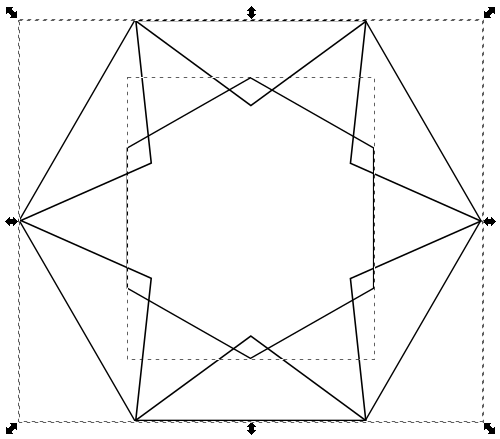
\includegraphics[width=1\linewidth]{3_1_create.png}} 
        Cоздание фигур\\
    \end{minipage}
    \hfill
    \begin{minipage}[h]{0.47\linewidth}
        \center{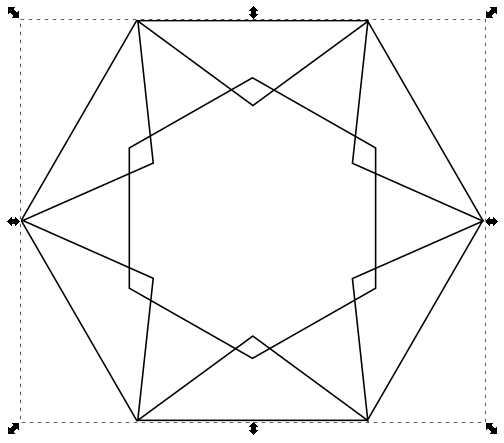
\includegraphics[width=1\linewidth]{3_2_exclusion.png}} 
        Операция Exclusion\\
    \end{minipage}
    \hfill
    \centering
    \begin{minipage}[h]{0.47\linewidth}
        \center{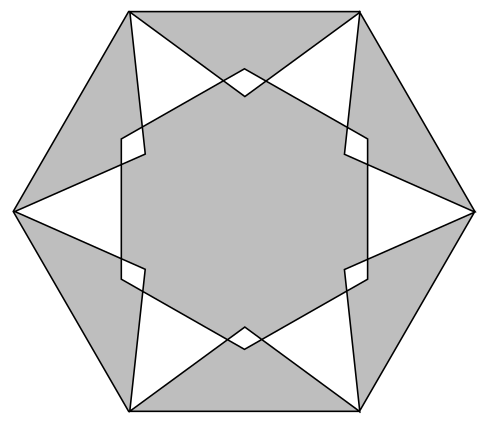
\includegraphics[width=1\linewidth]{3_3_fill.png}} 
        Fill and Stroke
    \end{minipage}
\end{figure}
